\documentclass[addpoints,12pt]{exam}
%\documentclass[12pt]{article}
\usepackage[letterpaper, margin=0.75in]{geometry}
\usepackage{graphicx}
\usepackage{enumitem}
\usepackage{booktabs}
\usepackage{tabularx}
\usepackage{amsmath
}
\begin{document}
\footer{}{Page \thepage\ of \numpages}{}

\begin{flushright}
\makebox[0.5\textwidth]{\large Name:\enspace\hrulefill}
\vspace{0.2in}

\makebox[0.5\textwidth]{\large Date:\enspace\hrulefill}
\end{flushright}

\begin{center}

\includegraphics[width=10cm]{../images/logo.png}
\end{center}

\begin{center}
\noindent{\LARGE Conceptual Physics \\ Homework Packet 2\\}
\end{center}
\noindent\begin{large}\textbf{Due: March 2, 2018}\end{large}
\vspace{0.2in}

Answer the questions in the spaces provided on the question sheets. If you run out of room for an answer, continue on the back of the page. If questions are taken from one of the textbooks, it will be indicated. A large portion of your grade will be calculated based on \textit{how} you obtained an answer, so please \textbf{show your work} (including all diagrams and drawings if relevant).

If you prefer working on loseleaf paper, or have a large portion of your work on loseleaf, please be sure to hand that in along with this homework packet.

The content in this homework relates to material we covered in class 3 (kinematics) and class 4 (graphs). Note that you will need use material from class 2 (units). The related readings are:
\begin{enumerate}
	\item \textit{Light and Matter}, Chapter 2 (Sections 1, 2 and 5)
	\item \textit{College Physics}, Chapter 2 (Sections 1 to 5)
	\item \textit{Light and Matter}, Chapter 2 (Section 3)
	\item \textit{College Physics}, Chapter 2 (Section 8)
	\item OPTIONAL: \textit{Light and Matter}, Chapter 3 (Sections 1 to 4, and 6)
\end{enumerate}

The following table of metric prefixes may be useful:
\vspace{0.2in}

\begin{tabularx}{\textwidth}{ X X X X X X }
	kilo & (none) & centi & mili & micro & nano \\
	k & (none) & c & m & $\mu$ & n \\
	$10^3$ & $10^0$ & $10^{-2}$ & $10^{-3}$ & $10^{-6}$ & $10^{-9}$ \\
	1000 & 1 & 0.01 & 0.001 & 0.000001 & 0.000000001 
\end{tabularx}
 
The following geometric relations may be useful:
\begin{enumerate}
	\item The circumference of a circle is calculated using the radius and number pi
	\begin{eqnarray}
	circumference = 2\times \pi \times radius = \pi \times diameter \nonumber
	\end{eqnarray}
	\item The area of a circle is calculated using the square of the radius and pi
	\begin{eqnarray}
	area = \pi \times r^2 \nonumber
	\end{eqnarray}
\end{enumerate} 
 
\clearpage

\begin{flushright}
Score: \hspace{0.2in} / \numpoints ~ points
\end{flushright}


\begin{questions}
\question[2]
Is it possible for speed to be constant while acceleration is not zero? If \textit{yes}, give an example. If \textit{no}, explain why not. (Feel free to include a diagram.)

From: \textit{College Physics,} Ch.2, Conceptual Question 13
\vspace{2in}

	\question[4]
	A car begins speeding up from rest, accelerating at a constant rate of $6~\text{m}/\text{s}^2$.
	\begin{parts}
		\part How long does it take to reach a velocity of 30 m/s?
			\vspace{1in}
		\part How far does it travel in this time?
			\vspace{1in}
	\end{parts}
	
	\question[4]
The North American and European continents, which are about 6000 km apart, are moving apart at a rate of about 2~cm/year.

\begin{parts}
\part Assuming this rate has remained constant since they began separating, when did they start separating?
\vspace{2in}

\clearpage
\part If new evidence was uncovered that the plates were steadily slowing down, how would this affect your answer (\textit{i.e.}, would it have taken more or less time for the plates to separate to their current distance)?
\vspace{1in}
\end{parts}

	\question[3]
	You are looking into a deep well. It is dark, and you cannot see the bottom. You want to find out how deep it is, so you drop a rock in, and you hear a splash 3.0 s later. How deep is the well? (For simplicity, let the acceleration due to gravity be $g=10~m/s^2$)
	
	From: \textit{Light and Matter,}	Ch. 3, Question 9
	\vspace{1.5in}

\question[4]
Your friend makes the following graphs of the \textbf{position} and \textbf{velocity} of an object as a function of time, but forgets to label the axes. He tells you the object was undergoing constant acceleration. Which plot is which? \textbf{Label the axes}. (Be sure to label both horizontal axis, as well as both vertical axis).
\noindent\begin{table}[h!]
     \begin{center}
     \begin{tabularx}{\textwidth}{ X X }
     
     (a) \raisebox{-\totalheight}{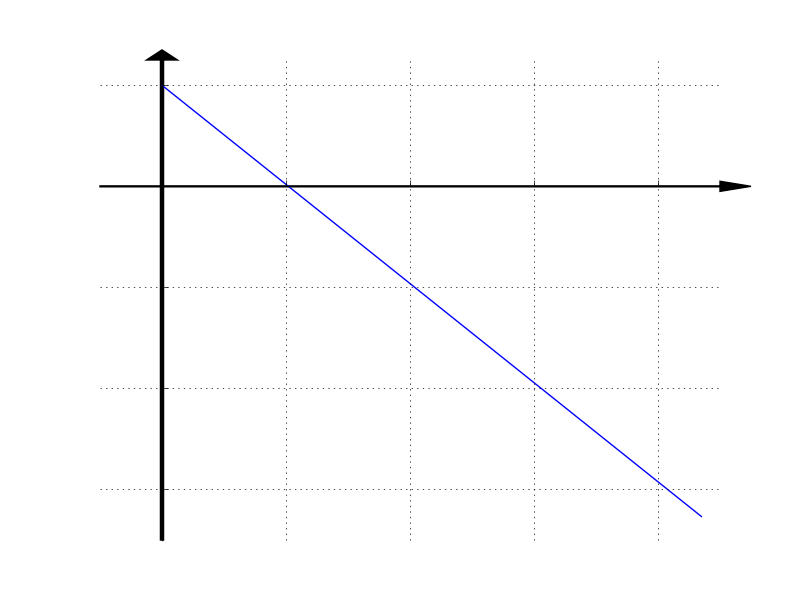
\includegraphics[width=0.45\textwidth]{../images/hw3_v.png}}
      & 
      (b) \raisebox{-\totalheight}{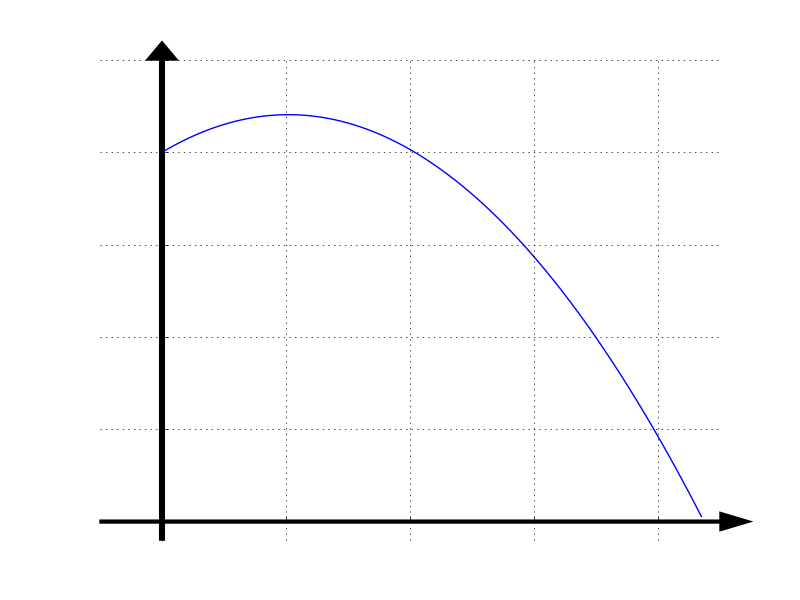
\includegraphics[width=0.45\textwidth]{../images/hw3_x.png}}\\
      \end{tabularx}
      \end{center}
\end{table}
	
\clearpage
	 \question[8]
You walk down a 10 m hallway at a constant speed in 10 s, pause for 5 s, then turn around and jog back to your initial position in another 5 s (again at a constant speed).
\begin{parts}
	\part Using the grid below, plot position as a function of time. Assume you begin walking at t=0 s.
	\begin{center}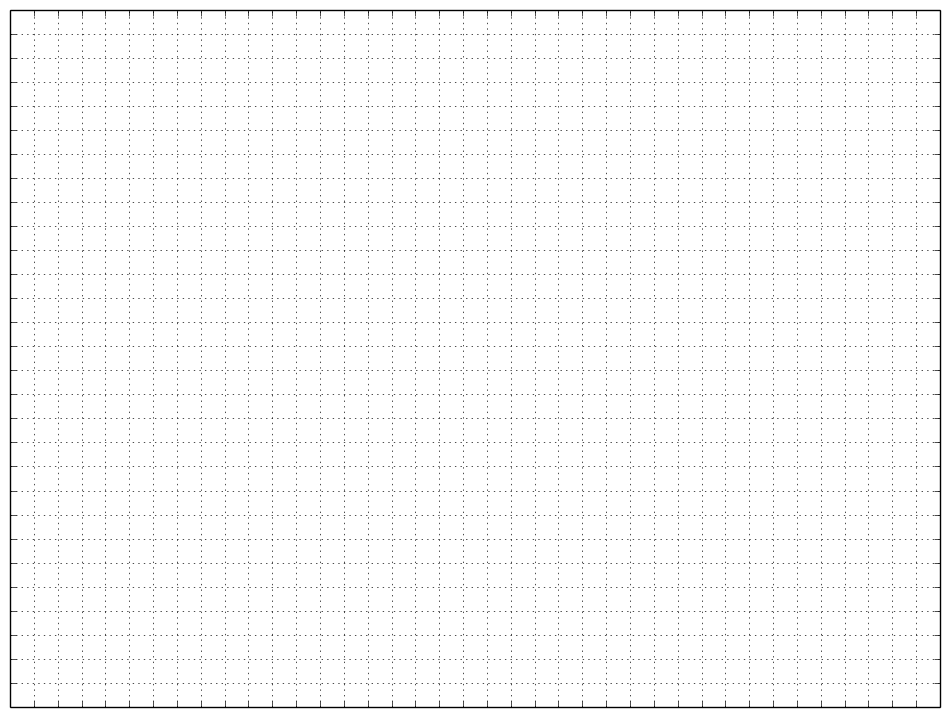
\includegraphics[width=0.75\textwidth]{../images/grid.png}\end{center}
	\part Using the grid below, plot velocity as a function of time. Assume you begin walking at t=0 s.
	\begin{center}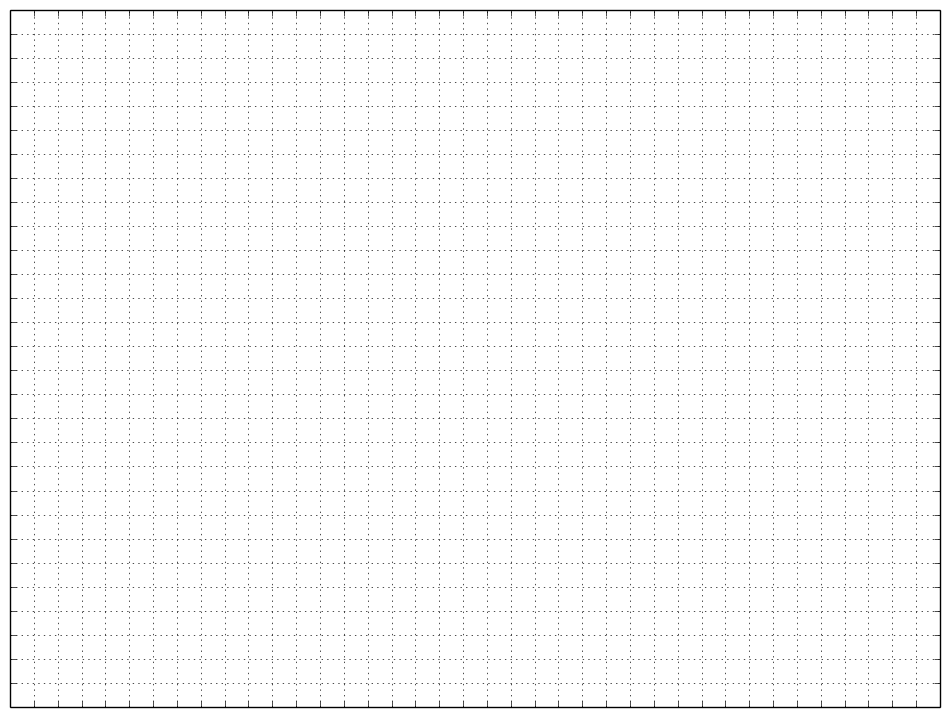
\includegraphics[width=0.75\textwidth]{../images/grid.png}\end{center}
	\part What is the distance traveled?
		\vspace{0.2in}
	\part What is you average speed?
		\vspace{0.2in}
	\part What is your displacement?
		\vspace{0.2in}
	\part What is your average velocity?
		\vspace{0.2in}
	\part What is your instantaneous velocity at t=5~s?
		\vspace{0.2in}
	\part What is your instantaneous velocity at t=18~s?
		\vspace{0.3in}
\end{parts}
	 
	 \bonusquestion[2]
Our Solar System is orbiting the center of the Milky Way Galaxy, which is about 28,000 light-years ($2.7\times 10^{17}$~km) away, in a roughly circular orbit.	 One orbit is called a galactic year and it takes about 250 million Earth years to complete.
\begin{parts}
\part What is the Solar System's average speed around the center of the galaxy? The answer can be in whatever units you're more comfortable with (km/s, miles/hour, km/year, etc.). A useful constant is $\pi = 3.14159... = 3$ (rounded for convenience).
	 \vspace{2in}
\end{parts}
	 
	 \begin{center}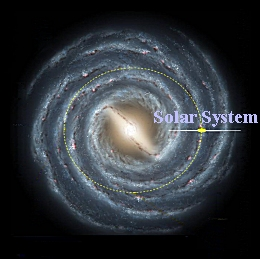
\includegraphics[width=0.4\linewidth]{../images/MilkyWaySolarSystem.jpg}\end{center}
	 
\end{questions}








\end{document}